\documentclass{ximera}

\title{Graphics, videos, and interactives}

\begin{document}
\begin{abstract}
  Embed compelling content in Ximera activities.
\end{abstract}
\maketitle

We've seen basic ways to include JPGs, PNGs, and PDFs using
\verb!\includegraphics!. However, this is not the preferred way to include
graphics. Moreover, there are considerations for positioning of the graphics.

\section{Positioning graphics}

In \LaTeX\ it is common to write images in the \verb!figure! environment. We
choose not to use this because \verb!figure! `floats' the images for `optimal'
page layout. We are not concerned with page layout. When working online, the
page is essentially infinite in length. Moreover, the \textit{consumers} of the
content we create are \textit{students}. Students are also unconcerned with
awkward page layout. Students prefer to see the image exactly when it is
mentioned. With this said, we suggest wrapping all images in either a
\verb!center! environment or an (Ximera-specific) \verb!image! environment.
The environment \verb!image! centers and automatically scales the contents.  If
an author finds themselves printing to various page-sizes, \verb!image! might
be preferred. Moreover, \verb!image! can be redefined globally to act
identically to \verb!center!, but \verb!center! cannot be redefined.

If you use \verb!center!, you would write something like:
\begin{verbatim}
\begin{center}

\includegraphics[width=5cm]{missionPatch.jpg}
\end{center}
\end{verbatim}
If you use \verb!image!, you would write something like:
\begin{verbatim}
\begin{center}

\includegraphics[width=5cm]{missionPatch.jpg}
\end{center}
\end{verbatim}

The disadvantage of using \verb!\includegraphics! is that you need to handle
the paths to the images in some way. You can do this by:
\begin{description}
  \item[Editing the graphics path]
  \item[Using a global graphics folder] can be done as follows by adding
\begin{verbatim}
\graphicspath{  %% When looking for inages,
{./}            %% look here first,
{./graphics/}   %% the look for a graphics folder,
{../graphics/}  %% which may be a directory up.
}
\end{verbatim}

Explain how to use a soft link to eat-your-cake and have-it too. 
You put the images in the folder with the source, then you soft link to the graphics directory. 
This is probably the best way to do it.


\end{description}
With this said, TikZ is the preferred method for graphics because code, found
in the Ximera \LaTeX\ file, generates the image. No need to worry about
graphics paths.

\section{TikZ is the preferred method for graphics}

The preferred way to include graphics is with TikZ.
\begin{image}
  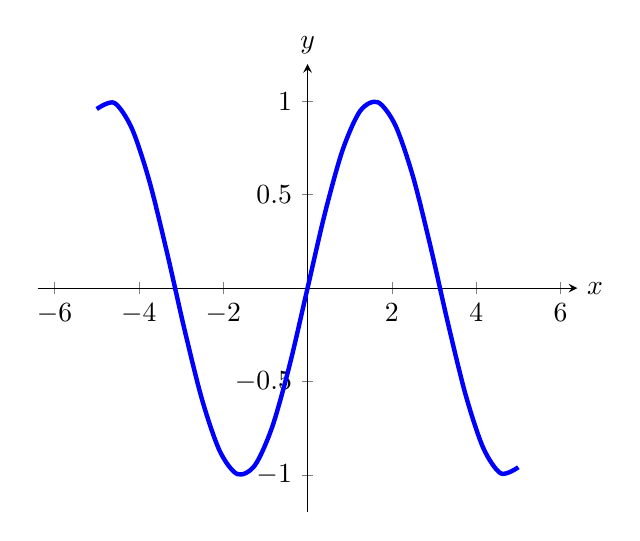
\begin{tikzpicture}
    \begin{axis}[
        xmin=-6.4,
        xmax=6.4,
        ymin=-1.2,
        ymax=1.2,
        axis lines=center,
        xlabel=$x$,
        ylabel=$y$,
        every axis y label/.style={at=(current axis.above
            origin),anchor=south},
        every axis x label/.style={at=(current axis.right of
            origin),anchor=west},
      ]
      \addplot [ultra thick, blue, smooth] {sin(deg(x))};
    \end{axis}
  \end{tikzpicture}
\end{image}

\begin{verbatim}
\begin{image}
  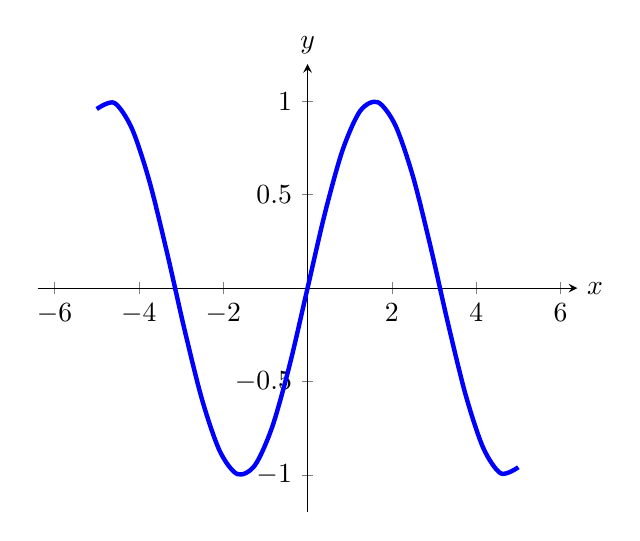
\begin{tikzpicture}
    \begin{axis}[
        xmin=-6.4,
        xmax=6.4,
        ymin=-1.2,
        ymax=1.2,
        axis lines=center,
        xlabel=$x$,
        ylabel=$y$,
        every axis y label/.style={at=(current axis.above origin),anchor=south},
        every axis x label/.style={at=(current axis.right of origin),anchor=west},
      ]
      \addplot [ultra thick, blue, smooth] {sin(deg(x))};
    \end{axis}
  \end{tikzpicture}
\end{image}
\end{verbatim}

\section{The graph command}

The easiest way to include an interactive graph is to use the
\verb|\graph| command. Unfortunately, the \verb|\graph| command
doesn't draw a graph in the PDF, rather, it states (in words) that a
graph is produced.
\begin{verbatim}
\graph{x^2,x^3}                     %% just x^2 and x^3
\graph{x^2 
\left\{ 1 \leq x \leq 10 \right\}}   %% restricted domain
\graph{\sin(x) \left\{x<0\right\}, 
2x \left\{ x>=0 \right\} }          %% piecewise
\graph{r=\theta} %% polar 
\end{verbatim}

\[
  \graph{x^2,x^3}
\]
There are a number of options for the \verb|\graph| command:



\paragraph{Change viewing window}
\[
  \graph[xmin=-5,xmax=5,ymin=-5,ymax=5]{y=x^2}
\]

\paragraph{Restricting domain}
\[
  \graph{x^2 \left\{ 1 \leq x \leq 10 \right\} }
\]
\paragraph{Restricting domain}
\[
  \graph{x^2 {1 \leq x \leq 10} }
\]
\paragraph{Graphing a piecewise function}

\begin{verbatim}
\[
\graph{ \sin(x)\left\{x<0\right\}, 2x\left\{ x>=0 \right\} }
\]
\end{verbatim}

\paragraph{Optional arguments for \texttt{\textbackslash graph}}

\begin{description}
  \item[\tt\bfseries xmin, ymin, xmax, ymax] These set the
    size of the viewing window with
    \verb|\graph[xmin=-5,xmax=5,ymin=-5,ymax=5]{y=x^2}|.
  \item[\tt\bfseries panel] Determines if the panel is shown with
    \verb|\graph[panel]{y=x^2}|.
  \item[\tt\bfseries xAxisLabel, yAxisLabel] Gives the axes labels with
    \verb|\graph[xAxisLabel="time", yAxisLabel="distance"]{y=x^2}|.
  \item[\tt\bfseries hideXAxis, hideYAxis] Hides the axes with
    \verb|\graph[hideXAxis=true, hideYAxis=true]{x^2}|.
  \item[\tt\bfseries hideXAxisNumbers=true, hideYAxisNumbers=true] Hides the tick marks on
    the axes with
    \verb|\graph[hideXAxisNumbers=true, hideYAxisNumbers=true]{y=x^2}|.
  \item[\tt\bfseries polar] Shows polar grid lines with \verb|\graph[polar]{y=x^2}|.
\end{description}

\[
  \graph{x^2 \left\{ 1 \leq x \leq 10 \right\}}
  \graph{ \sin(x)\left\{x<0\right\}, 2x\left\{ x>=0 \right\} }
\]
\section{Videos}

We can embed YouTube Videos with something like
\begin{verbatim}
\begin{center}
\youtube{FvgF95i0_lw}
\end{center}
\end{verbatim}
which would embed the video into the page, like this:
\begin{center}
  \youtube{FvgF95i0_lw}
\end{center}

\begin{warning}
  YouTube videos count toward the completion of the activity. As such,
  currently, students must watch the \textbf{entire} video to earn full credit.
\end{warning}

\section{Desmos, Desmos 3D, and GeoGebra}

If you require further features from
\link[Desmos]{https://www.desmos.com/}, you can sign up for an account
and include your worksheets like this:
\begin{verbatim}
\begin{center}
\desmos{zwywds7med}{800}{600}
\end{center}
\end{verbatim}
which renders as:
\begin{center}
  \desmos{zwywds7med}{800}{600}
\end{center}

The syntax for Desmos 3D is similar:
\begin{verbatim}
\begin{center}
\desmosThreeD{bb4exrhrl3}{800}{600}
\end{center}
\end{verbatim}
Seen here:
\begin{center}
  \desmosThreeD{bb4exrhrl3}{800}{600}
\end{center}

You can also use \link[GeoGebra]{https://www.geogebra.org/}. Embed the
widget using the syntax \verb|\geogebra{ID}{width}{height}|, where ID
is the widget ID and width and height are the dimensions (in pixels)
you want the embedded widget to have.
\begin{verbatim}
\begin{center}
\geogebra{XC3FXUdJ}{800}{600}
\end{center}
\end{verbatim}
\begin{center}
  \geogebra{XC3FXUdJ}{800}{600}%%https://www.geogebra.org/m/XC3FXUdJ
\end{center}

While we cannot get data from these sorts of interactives directly, the clever
author can ask questions that \textbf{use} the interactive to find a solution.

\end{document}